% subseccion 4.2
\subsection{Etapa 2: Búsqueda de Estudios}
Esta etapa presenta la estrategia de búsqueda usada en la revisión sistemática de la literatura. Esta estrategia se describe en detalle en las subsecciones~\ref{subsubsec:Definiendo la Estrategia de Busqueda} -- \ref{subsubsec:resultados-busqueda}. Ver figura~\ref{fig:etapa2}.

\begin{figure*}[tbp]
    \centering
    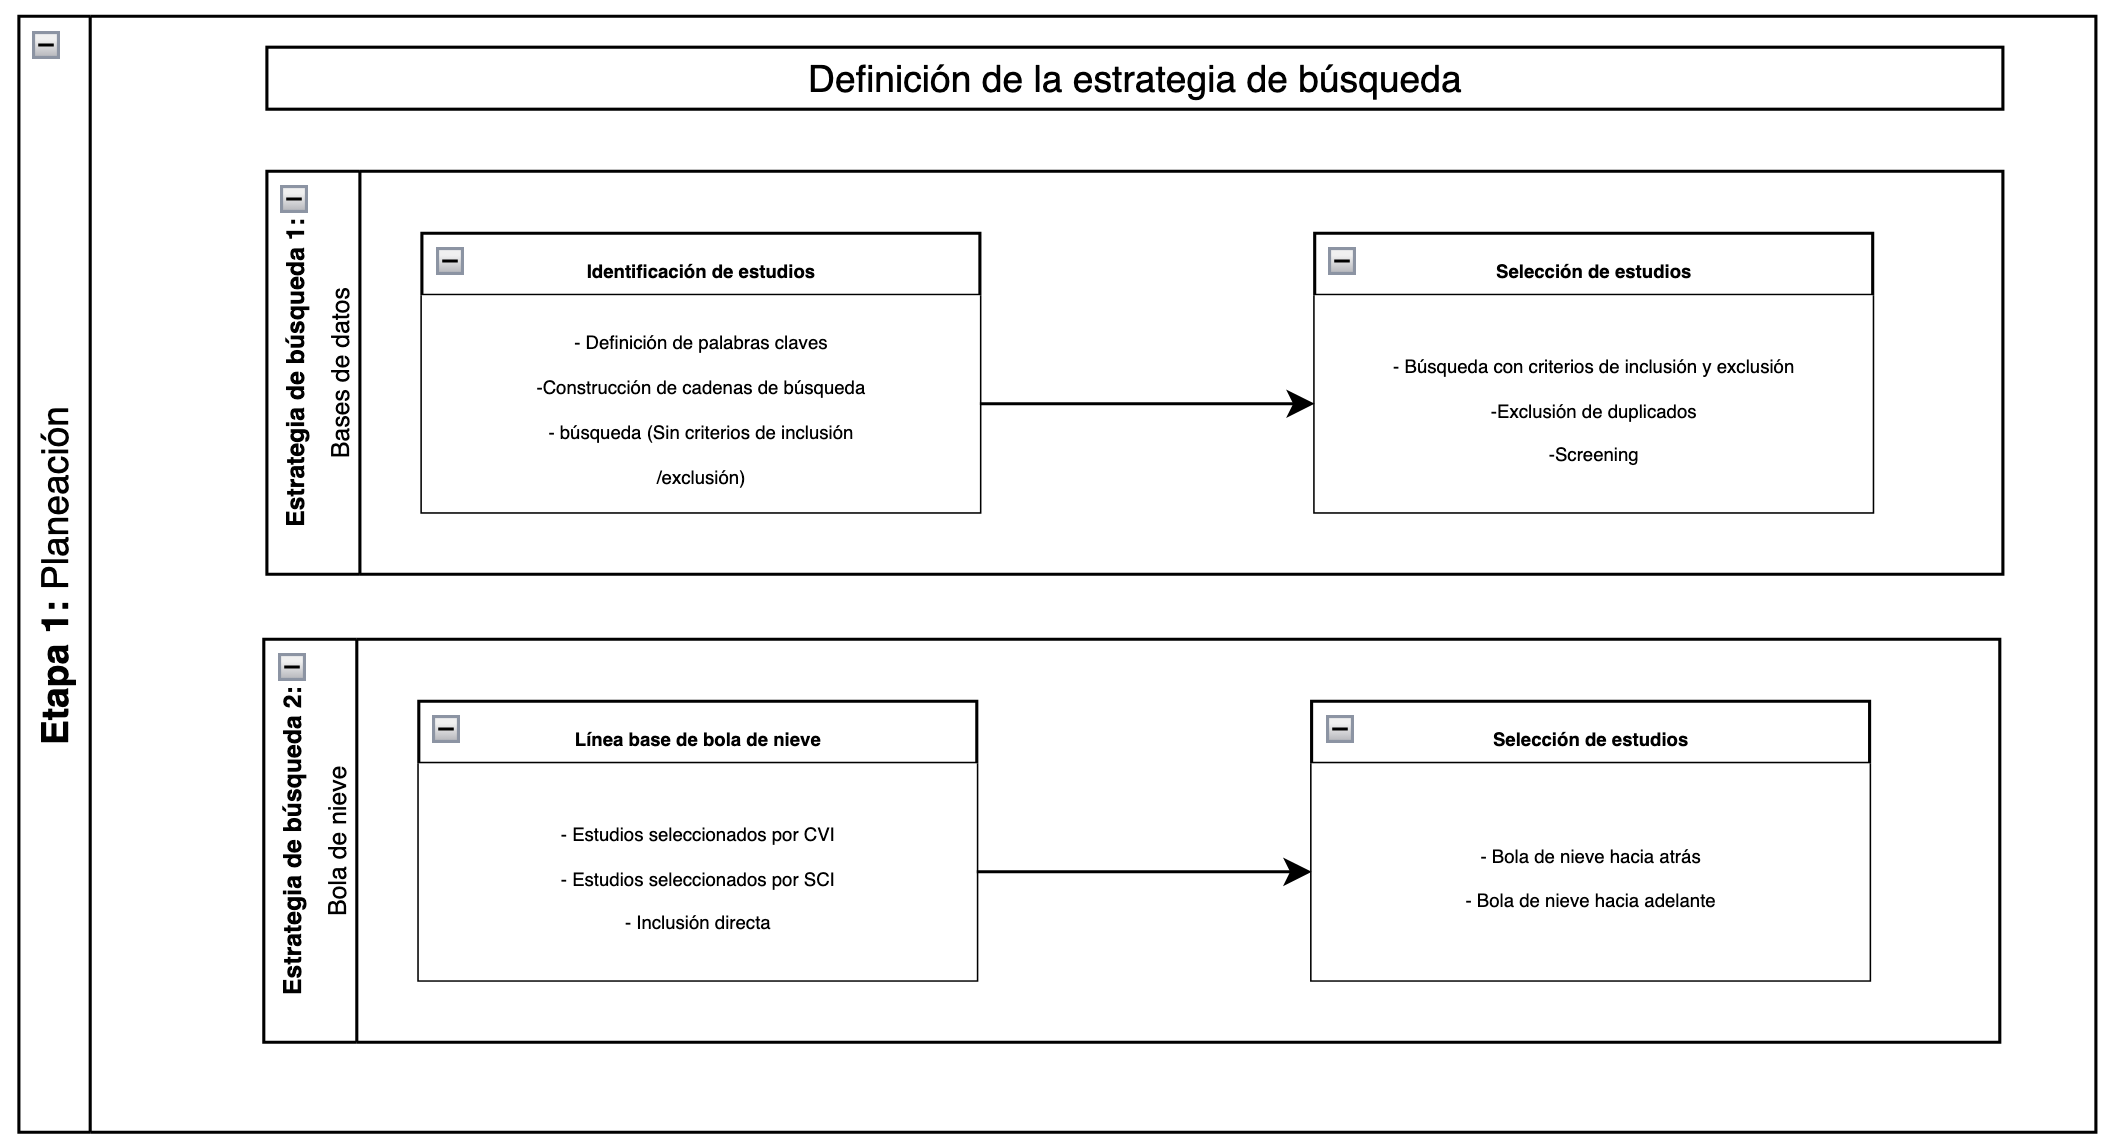
\includegraphics[width=0.8\textwidth]{resources/images/planeacion/estrategias-busqueda.png}
    \caption{Composición de la etapa de búsqueda de estudios}\label{fig:etapa2}
\end{figure*}
\mbox{}\\

%sub-subseccion 4.2.1 
\subsubsection{Definiendo la Estrategia de Búsqueda}\label{subsubsec:Definiendo la Estrategia de Busqueda}
\mbox{}\\
% Content for 4.2.1
Para la construcción de esta revisión de la literatura, se usó un enfoque híbrido. Con este enfoque se busca obtener mayor volumen de artículos indexados y con diferentes origenes. más allá de los proporcionados por las bases de datos.
En este sentido, se combinaron dos estrategias de búsqueda. La primer estrategia es la búsqueda en bases de datos y consiste en realizar una cadena de búsqueda automatizada en bases de datos académicas.~\cite{jalali2012systematic}.
La segunda estrategia es la denominada ``Bola de Nieve'' (Snowballing) y consiste en la búsqueda manual de artículos a partir de un conjunto base de artículos usando las referencias y las citas de los mismos. Esta estrategia se basa en la premisa de que los artículos relevantes citan otros artículos relevantes y, por lo tanto, permite encontrar artículos que no están indexados en las bases de datos académicas.~\cite{jalali2012systematic} y \cite{goodman1961snowball}.
\mbox{}\\
%sub-subseccion 4.2.2

\subsubsection{Estrategia de Búsqueda 1: Bases de Datos}
\mbox{}\\
Esta estrategia consta de 2 componentes. El primer componente es denominado ``Identificación de estudios''. Esto se enfoca en definir las palabras clave para construir las cadenas de búsqueda que conducen a completar las búsquedas en las bases de datos académicas.
El segundo componente es llamado ``Selección de estudios''. Se enfoca en aplicar varios criterios para refinar la búsqueda de resultados de estudios y así obtener el mayor valor del proceso de búsqueda. \\ \\

\begin{itemize}
    \item \textbf{Identificación de estudios:} En búsqueda de la viabilidad del estudio y por acuerdo de los autores, se limitó la búsqueda a cinco bases de datos académicas: \textit{ACM}, \textit{IEEE Xplore}, \textit{Springer}, \textit{Science Direct} y \textit{Taylor and Francis}. En esta parte del proceso es necesario establecer las palabras claves definidas antes y construir las cadenas de búsqueda específica para cada base de datos. Nuevamente se usó el modelo PICOC como guía metodológica para identificar términos claves o frases completas que se relacionan con las tecnologías de virtualización basadas en contenedores. En la construcción de estas cadenas de búsqueda se usaron sinónimos para ampliar el espectro de resultados. (Ver cuadro~\ref{tab:palabras-clave}).\\ 
    Las principales palabras clave identificadas fueron: \textit{Container-based virtualization}, \textit{Education}, \textit{Research}, \textit{Industry}. Para ampliar y refinar los resultados se usaron operadores booleanos como \textit{AND} y \textit{OR}. Además, se usaron comillas para buscar frases completas y paréntesis para agrupar términos relacionados. Finalmente, el conjunto de palabras clave seleccionadas para construir las cadenas de búsqueda se presenta en el cuadro~\ref{tab:keywords}.\\
    Para dirigir la búsqueda hacia la intercepción de los dominios de TI y la VBC se usó el operador booleano \textit{AND}. Una vez identificadas las palabras clave, se procedió con la construcción de las cadenas de búsqueda para cada base de datos, usando un proceso iterativo. El proceso de construcción de las cadenas de búsqueda consitió en realizar un proceso heúristico con las palabras clave, sinónimos y conceptos relacionados, haciendo uso de conjunciones y disyunciones conforme a las reglas de cada base de datos.\\ 
    Así, estas cadenas de búsqueda varían de acuerdo con las reglas de cada base de datos. Ver cuadro~\ref{tab:cadenas-busqueda}.\\

\end{itemize}

\begin{table}[tbp]
    \scriptsize % reduce tamaño del texto
    \centering
    \renewcommand{\arraystretch}{1.3}
    \begin{tabularx}{\columnwidth}{>{\centering\arraybackslash}m{0.18\columnwidth} >{\RaggedRight\arraybackslash}X}
        \hline
        \textbf{Aspecto} & \textbf{Descripción} \\
        \hline
        Población & VBC, Dominios de TI, Educación, Investigación, Extensión \\
        Intervención & Identificación, Clasificación \\
        Comparación & Tasa de éxito, Evidencia de uso \\
        Salida & Clasificación de trabajos relacionados con VBC en cada dominio de TI \\
        Contexto & Docencia, Investigación, Extensión \\
        \hline
    \end{tabularx}
    \caption{Palabras clave identificadas usando el modelo PICOC}\label{tab:palabras-clave}
\end{table}

\begin{table}[tbp]
    \scriptsize % reduce tamaño del texto
    \centering
    \renewcommand{\arraystretch}{1.3}
    \begin{tabularx}{\columnwidth}{>{\centering\arraybackslash}m{0.18\columnwidth} >{\RaggedRight\arraybackslash}X}
        \hline
        \textbf{Palabras clave} & \textbf{Sinónimos} \\
        \hline
        Container-based virtualization & Application virtualization, Docker, Lightweight Virtualization \\
        Education & Education System, Education Development, Higher Education \\
        Research & Research Group, Research Proposal \\
        Industry & IT Services, Technology Infrastructure, Cloud Computing \\
        \hline
    \end{tabularx}
    \caption{Palabras clave para la búsqueda en base de datos}\label{tab:keywords}
\end{table}




\newcolumntype{P}[1]{>{\raggedright\arraybackslash}p{#1}}

\begin{sidewaystable*}[htbp]
\centering
\scriptsize
\renewcommand{\arraystretch}{1.5}
\begin{adjustbox}{max width=\textwidth}
\begin{tabular}{|P{0.18\linewidth}|P{0.20\linewidth}|P{0.20\linewidth}|P{0.20\linewidth}|P{0.20\linewidth}|P{0.20\linewidth}|}
\hline
\textbf{Dominio / Base de Datos} & \textbf{ACM Digital Library} & \textbf{IEEE Xplore} & \textbf{ScienceDirect} & \textbf{SpringerLink}  & \textbf{Taylor \& Francis} \\
\hline
\textbf{Educación AND VBC} 
& \tiny \texttt{(Title:(``Container-based virtualization'' OR ``Application virtualization'' OR ``Docker'' OR ``Lightweight Virtualization'') AND Title:(``Education'' OR ``Education System'' OR ``Education Development'' OR ``Higher Education'')) OR (Abstract:(``Container-based virtualization'' OR ``Application virtualization'' OR ``Docker'' OR ``Lightweight Virtualization'') AND Abstract:(``Education'' OR ``Education System'' OR ``Education Development'' OR ``Higher Education'')) OR (Keyword:(``Container-based virtualization'' OR ``Application virtualization'' OR ``Docker'' OR ``Lightweight Virtualization'') AND Keyword:(``Education'' OR ``Education System'' OR ``Education Development'' OR ``Higher Education''))} 
& \tiny \texttt{((``Abstract'': ``Container-based virtualization'' OR ``Abstract'': ``Application virtualization'' OR ``Abstract'': ``Docker'' OR ``Abstract'': ``Lightweight Virtualization'') AND (``Abstract'': ``Education'' OR ``Abstract'': ``Education System'' OR ``Abstract'': ``Education Development''  OR ``Abstract'': ``Higher Education'')) OR ((``Publication Title'': ``Container-based virtualization'' OR ``Publication Title'': ``Application virtualization'' OR ``Publication Title'': ``Docker'' OR ``Publication Title'': ``Lightweight Virtualization'') AND (``Publication Title'': ``Education'' OR ``Publication Title'': ``Education System'' OR ``Publication Title'': ``Education Development''  OR ``Publication Title'': ``Higher Education'')) OR ((``Author Keywords'': ``Container-based virtualization'' OR ``Author Keywords'': ``Application virtualization'' OR ``Author Keywords'': ``Docker'' OR ``Author Keywords'': ``Lightweight Virtualization'') AND (``Author Keywords'': ``Education'' OR ``Author Keywords'': ``Education System'' OR ``Author Keywords'': ``Education Development''  OR ``Author Keywords'': ``Higher Education''))} 
& \tiny \texttt{(``Container-based virtualization'' OR ``Application virtualization'' OR ``Docker'' OR ``Lightweight Virtualization'') AND (``Education'' OR ``Education System'' OR ``Education Development'' OR ``Higher Education'')} 
& \tiny \texttt{(title:(``Container-based virtualization'' OR ``Application virtualization'' OR ``Docker'' OR ``Lightweight Virtualization'') AND title:(``Education'' OR ``Education System'' OR ``Education Development'' OR ``Higher Education'')) OR (abstract:(``Container-based virtualization'' OR ``Application virtualization'' OR ``Docker'' OR ``Lightweight Virtualization'') AND abstract:(``Education'' OR ``Education System'' OR ``Education Development'' OR ``Higher Education'')) OR (keyword:(``Container-based virtualization'' OR ``Application virtualization'' OR ``Docker'' OR ``Lightweight Virtualization'') AND keyword:(``Education'' OR ``Education System'' OR ``Education Development'' OR ``Higher Education''))} 
& \tiny \texttt{(``Application virtualization'' OR ``Docker'' OR ``Lightweight Virtualization'' OR ``Docker Container'') AND (``Education System'' OR ``Education Sector'' OR ``Education Development'' OR ``Higher Education'')} \\
\hline

\hline
\textbf{Investigación AND VBC}
& \tiny \texttt{(Title:(``Container-based virtualization'' OR ``Application virtualization'' OR ``Docker'' OR ``Lightweight Virtualization'') AND Title:(``Research'' OR ``Research Group'' OR ``Research Proposal'')) OR (Abstract:(``Container-based virtualization'' OR ``Application virtualization'' OR ``Docker'' OR ``Lightweight Virtualization'') AND Abstract:(``Research'' OR ``Research Group'' OR ``Research Proposal'')) OR (Keyword:(``Container-based virtualization'' OR ``Application virtualization'' OR ``Docker'' OR ``Lightweight Virtualization'') AND Keyword:(``Research'' OR ``Research Group'' OR ``Research Proposal''))} 
& \tiny \texttt{((``Abstract'': ``Container-based virtualization'' OR ``Abstract'': ``Application virtualization'' OR ``Abstract'': ``Docker'' OR ``Abstract'': ``Lightweight Virtualization'') AND (``Abstract'': ``Research Group'' OR ``Abstract'': ``Research Proposal'')) OR ((``Publication Title'': ``Container-based virtualization'' OR ``Publication Title'': ``Application virtualization'' OR ``Publication Title'': ``Docker'' OR ``Publication Title'': ``Lightweight Virtualization'') AND (``Publication Title'': ``Research Group'' OR ``Publication Title'': ``Research Proposal'')) OR ((``Author Keywords'': ``Container-based virtualization'' OR ``Author Keywords'': ``Application virtualization'' OR ``Author Keywords'': ``Docker'' OR ``Author Keywords'': ``Lightweight Virtualization'') AND (``Author Keywords'': ``Research Group'' OR ``Author Keywords'': ``Research Proposal''))} 
& \tiny \texttt{(``Container-based virtualization'' OR ``Application virtualization'' OR ``Docker'' OR ``Lightweight Virtualization'') AND (``Research'' OR ``Research Group'' OR ``Research Proposal'')} 
& \tiny \texttt{(title:(``Container-based virtualization'' OR ``Application virtualization'' OR ``Docker'' OR ``Lightweight Virtualization'') AND title:(``Research'' OR ``Research Group'' OR ``Research Proposal'')) OR (abstract:(``Container-based virtualization'' OR ``Application virtualization'' OR ``Docker'' OR ``Lightweight Virtualization'') AND abstract:(``Research'' OR ``Research Group'' OR ``Research Proposal'')) OR (keyword:(``Container-based virtualization'' OR ``Application virtualization'' OR ``Docker'' OR ``Lightweight Virtualization'') AND keyword:(``Research'' OR ``Research Group'' OR ``Research Proposal''))} 
& \tiny \texttt{(``Application virtualization'' OR ``Docker'' OR ``Lightweight Virtualization'' OR ``Docker Container'') AND (``Specific Research Areas'' OR ``Research Group'' OR ``Research Proposal'' OR ``Research and Development'')} \\
\hline

\hline
\textbf{Industria AND VBC}
& \tiny \texttt{(Title:(``Container-based virtualization'' OR ``Application virtualization'' OR ``Docker'' OR ``Lightweight Virtualization'') AND Title:(``Industry'' OR ``IT Services'' OR ``Technology Infrastructure'' OR ``Cloud Computing'')) OR (Abstract:(``Container-based virtualization'' OR ``Application virtualization'' OR ``Docker'' OR ``Lightweight Virtualization'') AND Abstract:(``Industry'' OR ``IT Services'' OR ``Technology Infrastructure'' OR ``Cloud Computing'')) OR (Keyword:(``Container-based virtualization'' OR ``Application virtualization'' OR ``Docker'' OR ``Lightweight Virtualization'') AND Keyword:(``Industry'' OR ``IT Services'' OR ``Technology Infrastructure'' OR ``Cloud Computing''))} 
& \tiny \texttt{((``Abstract'': ``Container-based virtualization'' OR ``Abstract'': ``Application virtualization'' OR ``Abstract'': ``Docker'' OR ``Abstract'': ``Lightweight Virtualization'') AND (``Abstract'': ``Industry'' OR ``Abstract'': ``IT Services'' OR ``Abstract'': ``Technology Infrastructure'' OR ``Abstract'': ``Cloud Computing'')) OR ((``Publication Title'': ``Container-based virtualization'' OR ``Publication Title'': ``Application virtualization'' OR ``Publication Title'': ``Docker'' OR ``Publication Title'': ``Lightweight Virtualization'') AND (``Publication Title'': ``Industry'' OR ``Publication Title'': ``IT Services'' OR ``Publication Title'': ``Technology Infrastructure'' OR ``Publication Title'': ``Cloud Computing'')) OR ((``Author Keywords'': ``Container-based virtualization'' OR ``Author Keywords'': ``Application virtualization'' OR ``Author Keywords'': ``Docker'' OR ``Author Keywords'': ``Lightweight Virtualization'') AND (``Author Keywords'': ``Industry'' OR ``Author Keywords'': ``IT Services'' OR ``Author Keywords'': ``Technology Infrastructure'' OR ``Author Keywords'': ``Cloud Computing''))} 
& \tiny \texttt{(``Container-based virtualization'' OR ``Application virtualization'' OR ``Docker'' OR ``Lightweight Virtualization'') AND (``Industry'' OR ``IT Services'' OR ``Technology Infrastructure'' OR ``Cloud Computing'')} 
& \tiny \texttt{(title:(``Container-based virtualization'' OR ``Application virtualization'' OR ``Docker'' OR ``Lightweight Virtualization'') AND title:(``Industry'' OR ``IT Services'' OR ``Technology Infrastructure'' OR ``Cloud Computing'')) OR (abstract:(``Container-based virtualization'' OR ``Application virtualization'' OR ``Docker'' OR ``Lightweight Virtualization'') AND abstract:(``Industry'' OR ``IT Services'' OR ``Technology Infrastructure'' OR ``Cloud Computing'')) OR (keyword:(``Container-based virtualization'' OR ``Application virtualization'' OR ``Docker'' OR ``Lightweight Virtualization'') AND keyword:(``Industry'' OR ``IT Services'' OR ``Technology Infrastructure'' OR ``Cloud Computing''))} 
& \tiny \texttt{(``Application virtualization'' OR ``Docker'' OR ``Lightweight Virtualization'' OR ``Docker Container'') AND (``Industry'' OR ``IT Services'' OR ``Technology Infrastructure'' OR ``Cloud Computing'')} \\
\hline
\end{tabular}
\end{adjustbox}
\caption{Cadenas de búsqueda por dominio y base de datos}\label{tab:cadenas-busqueda}
\end{sidewaystable*}










% sub-subsetion for 4.2.3
\subsubsection{Estrategia de Búsqueda 2: Bola de Nieve (Snowballing)}
Quis ut deserunt in nulla aliquip exercitation. Voluptate non laborum do eu dolor mollit officia cupidatat do ea id id ullamco. Dolore velit anim est pariatur eiusmod occaecat duis labore reprehenderit nisi esse. Eu laboris cillum ullamco non velit veniam labore eiusmod laboris sint. Consequat officia aliquip velit officia do ex nulla cupidatat elit dolore deserunt sint.
\mbox{}\\

% sub=-subsection 4.2.4
\subsubsection{Resultados de la Búsqueda de Estudios}
\label{subsubsec:resultados-busqueda}
Nostrud enim magna culpa labore in culpa aliqua dolore ea amet sit magna exercitation sunt. Voluptate qui aliqua velit ipsum ullamco dolor ad velit cupidatat dolore sint. Nisi cillum dolore magna tempor minim ullamco anim quis ipsum consequat officia.
\mbox{}\\